%----------------------------------------------------------------------------------------
%	PACKAGES AND THEMES
%----------------------------------------------------------------------------------------
\documentclass{beamer}
% Load a bunch of useful packages:
\usepackage{amssymb,amsmath,amsfonts,mathtools} % useful math fonts and symbols
\usepackage{geometry} % allows changing margins and sizes of stuff
\usepackage{hyperref} % allows referencing of lines of text, urls, figures etc
\usepackage{natbib} % allows citation referencing from a .bib file
\bibliographystyle{apalike} % American Psychological Association style guide
\usepackage{graphicx} % to include graphics from the figures folder with helpful formating options
\usepackage{tikz}
\usetikzlibrary{calc}
\definecolor{crimson}{RGB}{ 170, 4, 36 }
\definecolor{darkblue}{RGB}{ 4, 47, 170 }
\definecolor{brown}{RGB}{ 111, 71, 2 }
\definecolor{periwinkle}{RGB}{ 90, 177, 204 }
\definecolor{ducksgreen}{HTML}{007030}
%---------------------------------------------%
\usepackage{color} % custom color definitions:%
    %UOregon colors:                          %
    \definecolor{UOGreen}{RGB}{18, 71, 52}    %
    \definecolor{UOYellow}{RGB}{254, 225, 35} %
    %Secondary official colors:               %
    \definecolor{LegacyGreen}{HTML}{104735}   %
    \definecolor{GrassGreen}{HTML}{489D46}    %
    \definecolor{LimeGreen}{HTML}{8ABB40}     %
    \definecolor{Chartreuse}{HTML}{E2E11B}    %
    \definecolor{Berry}{HTML}{8D1D58}         %
    \definecolor{DarkBlue}{HTML}{004F6E}      %
    \definecolor{LightBlue}{HTML}{00A5B5}     %
%----------------------------------------------
\usepackage{setspace} % to specify single, double or one-half spacing of text
\usepackage{indentfirst} % indent first line of a text paragraph
\usepackage{multicol} %multipage ability
\usepackage{multirow}
\usepackage{ulem} % \ul (underline) command which will break over line ends
\usepackage{amsthm} % allows standarized theorem commands
\setbeamertemplate{theorems}[numbered]
\theoremstyle{plain}
\newtheorem{assume}{Assumption}
\newtheorem{define}{Definition}
\usepackage{breqn} %automatic line breaking
\normalem

% Theming and Appearance Setup:
\usetheme{metropolis}
\metroset{block=fill}
%\usetheme{default}
\usefonttheme{professionalfonts}
\fontfamily{ppl}\selectfont
\usecolortheme[named=UOGreen]{structure}
\setbeamertemplate{footline}[frame number]
\setbeamertemplate{headline}{} %Removes Section Index on top of slide
\beamertemplatenavigationsymbolsempty
\hypersetup{
    colorlinks=true,
    linkcolor=DarkBlue,
    filecolor=Berry,
    citecolor=GrassGreen,
    urlcolor={LightBlue},
    pdftitle={Trade and Labor Market Dynamics},
    pdfpagemode=FullScreen
}

%----------------------------------------------------------------------------------------
%	TITLE PAGE
%----------------------------------------------------------------------------------------

% The title
\title{Combining Simultaneous \& Sequential Moves}
\author{Dante Yasui}
%\institute{University of Oregon}
\date{Winter 2024}
\titlegraphic{
\includegraphics[scale=.4]{UOSignature-356.png}}


%----------------------------------------------------------------------------------------
%	PRESENTATION SLIDES
%----------------------------------------------------------------------------------------

\begin{document}

\begin{frame}[plain]
    % Print the title page as the first slide
    \titlepage
\end{frame}
\addtocounter{framenumber}{-1}

\begin{frame}{Outline}
  \tableofcontents
\end{frame}

% - - - - - - - - - - - - - - - - - - - - - - - - - - - - - - - - - - - - - - -
\section{Games with both types of moves}

\begin{frame}
  \begin{itemize}

    \item So far, we have only seen games that were either made up of 
    \textit{only sequential} or \textit{only simultaneous} moves.

    \item But realistically, 
    many strategic interactions will contain both types of moves.

    \item Learning to move between extensive and strategic form 
    will help us examine more complicated games,
    as well as introduce us to the roll of \textit{information} and beliefs
    which will become useful to later topics.

  \end{itemize}
\end{frame}

% - - - - - - - - - - - - - - - - - - - - - - - - - - - - - - - - - - - - - - -

\begin{frame}{Original Kidnap Game}
  \begin{center}
    \documentclass[border=3mm, tikz]{standalone}
\usepackage{graphicx,tikz} % Required for inserting images
\usetikzlibrary{calc}
\usepackage{xcolor}
\definecolor{crimson}{RGB}{ 170, 4, 36 }
\definecolor{darkblue}{RGB}{ 4, 47, 170 }
\begin{document}

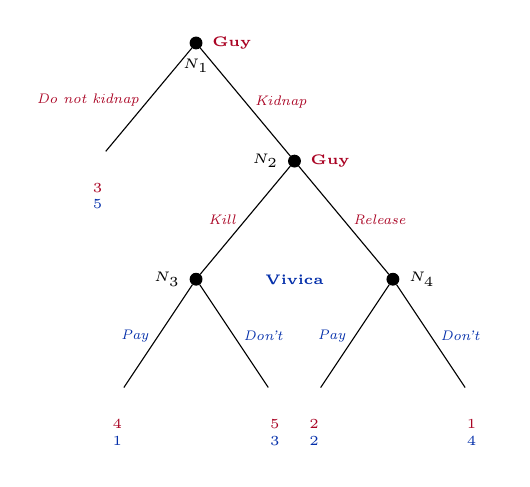
\begin{tikzpicture}[scale=1.0,font=\tiny]
\tikzstyle{solid node}=[circle,draw,inner sep=1.5,fill=black]
\tikzstyle{level 1}=[level distance=15mm,sibling distance=2.5cm]
\tikzstyle{level 2}=[level distance=15mm,sibling distance=2.5cm]
\tikzstyle{level 3}=[level distance=15mm,sibling distance=2cm]

\node(0)[solid node,label=right:{\textbf{\color{crimson} Guy}}, label=below:{$N_1$}]{}
    child{node[label=below:{
            \begin{tabular}{c}
                 {\color{crimson}  3} \\
                 {\color{darkblue} 5} \\
            \end{tabular}
        }
        ]{} 
    edge from parent node[left]{\textit{\color{crimson} Do not kidnap}}
    }
    child{node[solid node,label=right:{\textbf{\color{crimson} Guy}},
                          label=left:{$N_2$}]{} 
        child{node(1)[solid node, label=left:{$N_3$}]{} 
            child{node[label=below:{ 
                \begin{tabular}{c}
                     {\color{crimson}  4} \\
                     {\color{darkblue} 1} \\
                \end{tabular}
                }]{} 
            edge from parent node[left]{\textit{\color{darkblue} Pay}} 
            }
            child{node[label=below:{ 
                \begin{tabular}{c}
                     {\color{crimson}  5} \\
                     {\color{darkblue} 3} \\
                \end{tabular}
                }]{} 
            edge from parent node[right]{\textit{\color{darkblue} Don't}} 
            }
        edge from parent node[left]{\textit{\color{crimson} Kill}} 
        }
        child{node(2)[solid node, label=right:{$N_4$}]{} 
            child{node[label=below:{
                \begin{tabular}{c}
                    {\color{crimson}  2} \\
                    {\color{darkblue} 2} \\
                \end{tabular}
                }]{} 
            edge from parent node[left]{\textit{\color{darkblue} Pay}} 
            }
            child{node[label=below:{
                \begin{tabular}{c}
                     {\color{crimson}  1} \\
                     {\color{darkblue} 4} \\
                \end{tabular}
            }]{} 
            edge from parent node[right]{\textit{\color{darkblue} Don't}} 
            }
        edge from parent node[right]{\textit{\color{crimson} Release}} 
        }
    edge from parent node[right]{\textit{\color{crimson} Kidnap}}
    };

% information set
% \draw[dashed,rounded corners=10]($(1) + (-.2,.25)$)rectangle($(2) +(.2,-.25)$);
% specify mover at 2nd information set
\node at ($(1)!.5!(2)$) {\textbf{\color{darkblue} Vivica}};
% label info set
% \node at ($(1)!.5!(2) + (0,.35)$) {\textit{Info. Set}};


    
\end{tikzpicture}
\end{document}

  \end{center}
\end{frame}

% - - - - - - - - - - - - - - - - - - - - - - - - - - - - - - - - - - - - - - -

\begin{frame}{Modifying the game}
  \begin{itemize}

    \item When we first saw this game,
    Vivica could observe whether Guy had killed Orlando before she paid the ransom. 

    \item Now we will consider a variation of this game 
    where Orlando's fate is decided by Guy 
    \textit{without Vivica knowing the result}.

  \end{itemize}
\end{frame}

% - - - - - - - - - - - - - - - - - - - - - - - - - - - - - - - - - - - - - - -

\begin{frame}{Kidnap Game with a simultaneous subgame}
  \begin{center}
    \documentclass[border=3mm, tikz]{standalone}
\usepackage{graphicx,tikz} % Required for inserting images
\usetikzlibrary{calc}
\usepackage{xcolor}
\definecolor{crimson}{RGB}{ 170, 4, 36 }
\definecolor{darkblue}{RGB}{ 4, 47, 170 }
\begin{document}

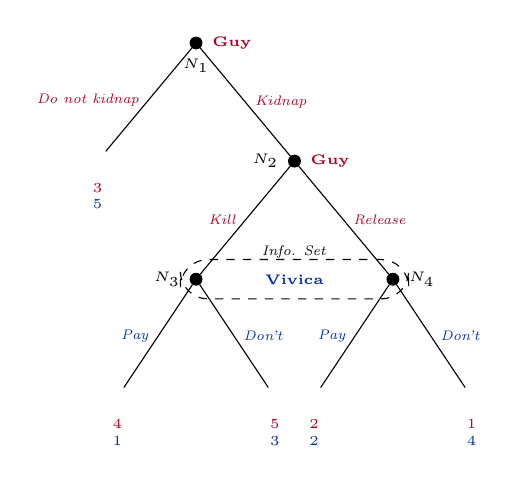
\begin{tikzpicture}[scale=1.0,font=\tiny]
\tikzstyle{solid node}=[circle,draw,inner sep=1.5,fill=black]
\tikzstyle{level 1}=[level distance=15mm,sibling distance=2.5cm]
\tikzstyle{level 2}=[level distance=15mm,sibling distance=2.5cm]
\tikzstyle{level 3}=[level distance=15mm,sibling distance=2cm]

\node(0)[solid node,label=right:{\textbf{\color{crimson} Guy}}, label=below:{$N_1$}]{}
    child{node[label=below:{
            \begin{tabular}{c}
                 {\color{crimson}  3} \\
                 {\color{darkblue} 5} \\
            \end{tabular}
        }
        ]{} 
    edge from parent node[left]{\textit{\color{crimson} Do not kidnap}}
    }
    child{node[solid node,label=right:{\textbf{\color{crimson} Guy}},
                          label=left:{$N_2$}]{} 
        child{node(1)[solid node, label=left:{$N_3$}]{} 
            child{node[label=below:{ 
                \begin{tabular}{c}
                     {\color{crimson}  4} \\
                     {\color{darkblue} 1} \\
                \end{tabular}
                }]{} 
            edge from parent node[left]{\textit{\color{darkblue} Pay}} 
            }
            child{node[label=below:{ 
                \begin{tabular}{c}
                     {\color{crimson}  5} \\
                     {\color{darkblue} 3} \\
                \end{tabular}
                }]{} 
            edge from parent node[right]{\textit{\color{darkblue} Don't}} 
            }
        edge from parent node[left]{\textit{\color{crimson} Kill}} 
        }
        child{node(2)[solid node, label=right:{$N_4$}]{} 
            child{node[label=below:{
                \begin{tabular}{c}
                    {\color{crimson}  2} \\
                    {\color{darkblue} 2} \\
                \end{tabular}
                }]{} 
            edge from parent node[left]{\textit{\color{darkblue} Pay}} 
            }
            child{node[label=below:{
                \begin{tabular}{c}
                     {\color{crimson}  1} \\
                     {\color{darkblue} 4} \\
                \end{tabular}
            }]{} 
            edge from parent node[right]{\textit{\color{darkblue} Don't}} 
            }
        edge from parent node[right]{\textit{\color{crimson} Release}} 
        }
    edge from parent node[right]{\textit{\color{crimson} Kidnap}}
    };

% information set
\draw[dashed,rounded corners=10]($(1) + (-.2,.25)$)rectangle($(2) +(.2,-.25)$);
% specify mover at 2nd information set
\node at ($(1)!.5!(2)$) {\textbf{\color{darkblue} Vivica}};
% label info set
\node at ($(1)!.5!(2) + (0,.35)$) {\textit{Info. Set}};


\end{tikzpicture}
\end{document}

  \end{center}
\end{frame}

% - - - - - - - - - - - - - - - - - - - - - - - - - - - - - - - - - - - - - - -

\begin{frame}
  \begin{itemize}

    \item The dotted box around Vivica's nodes $N_3$ and $N_4$
    indicate that she can't tell them apart.

    \item They are part of the same \alert{information set}; 
    to Vivica, they are indistinguishable from each other.

    \begin{definition}
      An \textit{information set} 
      is the set of information available to a player when making a decision. 
      In the extensive form, 
      every decision node belongs to one and only one info set,
      but multiple nodes may be in the same info set 
      if the player at that node cannot tell them apart.
    \end{definition}

  \end{itemize}
\end{frame}

% - - - - - - - - - - - - - - - - - - - - - - - - - - - - - - - - - - - - - - -
\section{Combining Sequential and Strategic Form}
\begin{frame}{Using Strategic Form in Extensive Games}

  Consider the situation when Guy has already kidnapped Orlando.

  List the remaining strategies for each player:
  
\end{frame}

% - - - - - - - - - - - - - - - - - - - - - - - - - - - - - - - - - - - - - - -

\begin{frame}{Using Strategic Form in Extensive Games}

  With these strategy profiles,
  we can write this subgame out in its strategic form:

  \begin{table}
  \centering
	  \begin{tabular}{cc|c|c|}
	  	& \multicolumn{1}{c}{} & \multicolumn{2}{c}{Vivica}\\
	  	& \multicolumn{1}{c}{} & \multicolumn{1}{c}{$Pay$}  & \multicolumn{1}{c}{$Dont~Pay$} \\\cline{3-4}
      \multirow{2}{*}{Guy}  & $Kill$ & $4,1$ & $2,2$ \\\cline{3-4}
	  	& $Release$ & $5,3$ & $1,4$ \\\cline{3-4}
	  \end{tabular}
  \end{table}

\end{frame}

% - - - - - - - - - - - - - - - - - - - - - - - - - - - - - - - - - - - - - - -

\begin{frame}{Going from Strategic to Extensive}
  
  For every strategic form game, 
  there are multiple extensive form game trees
  which can be drawn.

\end{frame}

% - - - - - - - - - - - - - - - - - - - - - - - - - - - - - - - - - - - - - - -

\begin{frame}{Two extensive subgames}
  \begin{minipage}{.4\textwidth}
    \centering
    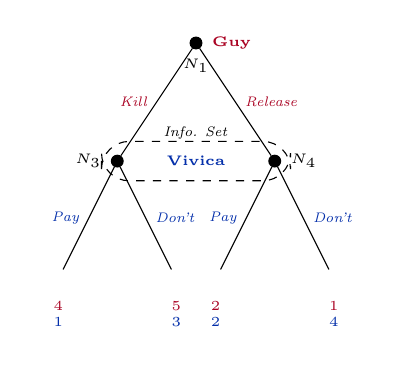
\begin{tikzpicture}[scale=1.0,font=\tiny]
\tikzstyle{solid node}=[circle,draw,inner sep=1.5,fill=black]
\tikzstyle{level 1}=[level distance=15mm,sibling distance=2cm]
\tikzstyle{level 2}=[level distance=15mm,sibling distance=1.5cm]
\tikzstyle{level 3}=[level distance=15mm,sibling distance=1cm]

\node(0)[solid node,label=right:{\textbf{\color{crimson} Guy}}, label=below:{$N_1$}]{}
  child{node(1)[solid node, label=left:{$N_3$}]{} 
      child{node[label=below:{ 
          \begin{tabular}{c}
               {\color{crimson}  4} \\
               {\color{darkblue} 1} \\
          \end{tabular}
          }]{} 
      edge from parent node[left]{\textit{\color{darkblue} Pay}} 
      }
      child{node[label=below:{ 
          \begin{tabular}{c}
               {\color{crimson}  5} \\
               {\color{darkblue} 3} \\
          \end{tabular}
          }]{} 
      edge from parent node[right]{\textit{\color{darkblue} Don't}} 
      }
  edge from parent node[left]{\textit{\color{crimson} Kill}} 
  }
  child{node(2)[solid node, label=right:{$N_4$}]{} 
      child{node[label=below:{
          \begin{tabular}{c}
              {\color{crimson}  2} \\
              {\color{darkblue} 2} \\
          \end{tabular}
          }]{} 
      edge from parent node[left]{\textit{\color{darkblue} Pay}} 
      }
      child{node[label=below:{
          \begin{tabular}{c}
               {\color{crimson}  1} \\
               {\color{darkblue} 4} \\
          \end{tabular}
      }]{} 
      edge from parent node[right]{\textit{\color{darkblue} Don't}} 
      }
  edge from parent node[right]{\textit{\color{crimson} Release}} 
  };

% information set
\draw[dashed,rounded corners=10]($(1) + (-.2,.25)$)rectangle($(2) +(.2,-.25)$);
% specify mover at 2nd information set
\node at ($(1)!.5!(2)$) {\textbf{\color{darkblue} Vivica}};
% label info set
\node at ($(1)!.5!(2) + (0,.35)$) {\textit{Info. Set}};


    
\end{tikzpicture}

  \end{minipage}
  \begin{minipage}{.4\textwidth}
    \centering
    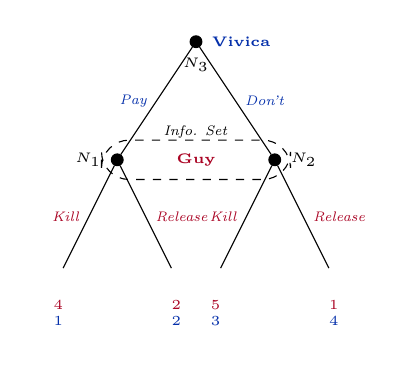
\begin{tikzpicture}[scale=1.0,font=\tiny]
\tikzstyle{solid node}=[circle,draw,inner sep=1.5,fill=black]
\tikzstyle{level 1}=[level distance=15mm,sibling distance=2cm]
\tikzstyle{level 2}=[level distance=15mm,sibling distance=1.5cm]
\tikzstyle{level 3}=[level distance=15mm,sibling distance=1cm]

\node(0)[solid node,label=right:{\textbf{\color{darkblue} Vivica}}, label=below:{$N_3$}]{}
  child{node(1)[solid node, label=left:{$N_1$}]{} 
      child{node[label=below:{ 
          \begin{tabular}{c}
               {\color{crimson}  4} \\
               {\color{darkblue} 1} \\
          \end{tabular}
          }]{} 
      edge from parent node[left]{\textit{\color{crimson} Kill}} 
      }
      child{node[label=below:{ 
          \begin{tabular}{c}
               {\color{crimson}  2} \\
               {\color{darkblue} 2} \\
          \end{tabular}
          }]{} 
      edge from parent node[right]{\textit{\color{crimson} Release}} 
      }
  edge from parent node[left]{\textit{\color{darkblue} Pay}} 
  }
  child{node(2)[solid node, label=right:{$N_2$}]{} 
      child{node[label=below:{
          \begin{tabular}{c}
              {\color{crimson}  5} \\
              {\color{darkblue} 3} \\
          \end{tabular}
          }]{} 
      edge from parent node[left]{\textit{\color{crimson} Kill}} 
      }
      child{node[label=below:{
          \begin{tabular}{c}
               {\color{crimson}  1} \\
               {\color{darkblue} 4} \\
          \end{tabular}
      }]{} 
      edge from parent node[right]{\textit{\color{crimson} Release}} 
      }
  edge from parent node[right]{\textit{\color{darkblue} Don't }} 
  };

% information set
\draw[dashed,rounded corners=10]($(1) + (-.2,.25)$)rectangle($(2) +(.2,-.25)$);
% specify mover at 2nd information set
\node at ($(1)!.5!(2)$) {\textbf{\color{crimson} Guy}};
% label info set
\node at ($(1)!.5!(2) + (0,.35)$) {\textit{Info. Set}};


    
\end{tikzpicture}

  \end{minipage}
\end{frame}

% - - - - - - - - - - - - - - - - - - - - - - - - - - - - - - - - - - - - - - -

\begin{frame}{Another way to represent the entire Kidnap Game}
  \begin{center}
    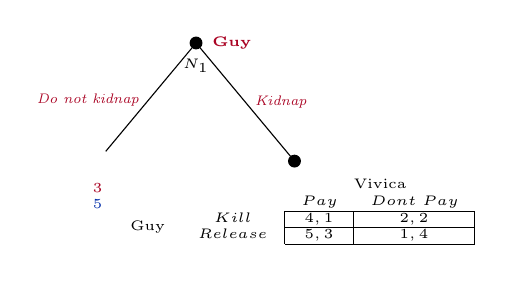
\begin{tikzpicture}[scale=1.0,font=\tiny]
\tikzstyle{solid node}=[circle,draw,inner sep=1.5,fill=black]
\tikzstyle{level 1}=[level distance=15mm,sibling distance=2.5cm]
\tikzstyle{level 2}=[level distance=15mm,sibling distance=2.5cm]
\tikzstyle{level 3}=[level distance=15mm,sibling distance=2cm]

\node(0)[solid node,label=right:{\textbf{\color{crimson} Guy}}, label=below:{$N_1$}]{}
    child{node[label=below:{
            \begin{tabular}{c}
                 {\color{crimson}  3} \\
                 {\color{darkblue} 5} \\
            \end{tabular}
        }
        ]{} 
    edge from parent node[left]{\textit{\color{crimson} Do not kidnap}}
    }
    child{node[solid node,label=below:{
      \begin{tabular}{cc|c|c|}
	  	& \multicolumn{1}{c}{} & \multicolumn{2}{c}{Vivica}\\
	  	& \multicolumn{1}{c}{} & \multicolumn{1}{c}{$Pay$}  & \multicolumn{1}{c}{$Dont~Pay$} \\\cline{3-4}
      \multirow{2}{*}{Guy}  & $Kill$ & $4,1$ & $2,2$ \\\cline{3-4}
	  	& $Release$ & $5,3$ & $1,4$ \\\cline{3-4}
	  \end{tabular}
    }]{} 
    edge from parent node[right]{\textit{\color{crimson} Kidnap}}
    };

% information set
% \draw[dashed,rounded corners=10]($(1) + (-.2,.25)$)rectangle($(2) +(.2,-.25)$);
% specify mover at 2nd information set
% \node at ($(1)!.5!(2)$) {\textbf{\color{darkblue} Vivica}};
% label info set
% \node at ($(1)!.5!(2) + (0,.35)$) {\textit{Info. Set}};


    
\end{tikzpicture}

  \end{center}
\end{frame}

% - - - - - - - - - - - - - - - - - - - - - - - - - - - - - - - - - - - - - - -

\begin{frame}{A Strategic Form representation}
  \begin{table}[h]
  \centering
    \begin{tabular}{cc|c|c|c|c|}
	  	& \multicolumn{1}{c}{} & \multicolumn{4}{c}{Guy}\\
      & \multicolumn{1}{c}{} & \multicolumn{1}{c}{$dnk,k$}  & \multicolumn{1}{c}{$dnk,r$} & \multicolumn{1}{c}{$kid,k$} & \multicolumn{1}{c}{$kid,r$} \\\cline{3-6}
      \multirow{2}{*}{Vivica}  & $pay$ & $5,3$ & $5,3$ & $1,4$ & $3,5$ \\\cline{3-6}
      & $no~pay$ & $5,3$ & $5,3$ & $2,2$ & $4,1$ \\\cline{3-6}
	  \end{tabular}

  \end{table}
\end{frame}

% - - - - - - - - - - - - - - - - - - - - - - - - - - - - - - - - - - - - - - -
\section{SPNE vs NE}


\begin{frame}
\frametitle{Market Entry Game}
\begin{itemize}
\item Consider this variation on the Entry Game, in which the Entrant is not as efficient as the Incumbent:
\end{itemize}
\begin{figure}
	\begin{minipage}{0.49\linewidth}
		\centering
		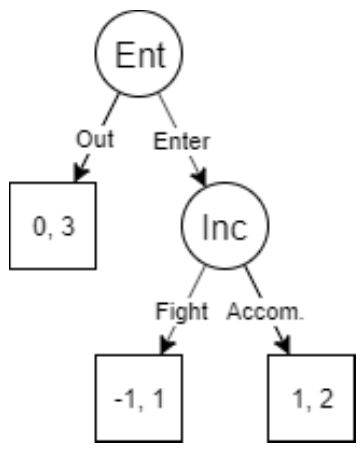
\includegraphics[width=0.55\textwidth]{figures/08InferiorEntrant.png}
	\end{minipage}
	\begin{minipage}{0.49\linewidth}
		\begin{tabular}{cc|c|c|}
			& \multicolumn{1}{c}{} & \multicolumn{2}{c}{Incumbent}\\
			& \multicolumn{1}{c}{} & \multicolumn{1}{c}{$Fight$}  & \multicolumn{1}{c}{$Accom.$} \\\cline{3-4}
			\multirow{2}*{Entrant}  & $Enter$ & -1, 1 & 1, 2 \\\cline{3-4}
			& $Out$ & 0, 3 & 0, 3 \\\cline{3-4}
		\end{tabular}
	\end{minipage}
\end{figure}
\begin{itemize}
\item Note that this game has two NEs: (Enter, Accommodate) and (Out, Fight). 
\item Does it really make sense for the Incumbent to ever Fight?
\end{itemize}
\end{frame}

\begin{frame}
\frametitle{Refining Nash Equilibrium}
\begin{itemize}
\item The more you think about it, the less sense this Nash equilibrium makes.
\item The only reason why the Entrant would choose to stay Out is if they really, truly believe that if they Entered, the Incumbent would Fight.
\item \dots but it's hard to justify that belief when Fighting is costly for the Incumbent.
\begin{itemize}
\item The Incumbent would have to somehow convince the Entrant that they really would Fight them, perhaps by making a \alert{credible threat}.
\item We will talk more about this kind of \alert{strategic move} later in the course.
\end{itemize}
\item We often don't want this kind of Nash Equilibrium. To rule it out, we have the concept of \alert{subgame perfection}.
\end{itemize}
\end{frame}

\begin{frame}
\frametitle{Subgames}
\begin{itemize}
\item A \alert{subgame} is a subset of an extensive-form game which, itself, is a complete game.
\item In the context of a game tree, a subgame is a \textbf{single node}, and all of the branches and nodes descending from it, such that it forms a complete game.
\end{itemize}
\end{frame}

\begin{frame}
\frametitle{Examples of Subgames}
\begin{itemize}
\item Each of these green boxes contains a subgame.
\end{itemize}
\begin{figure}
\centering
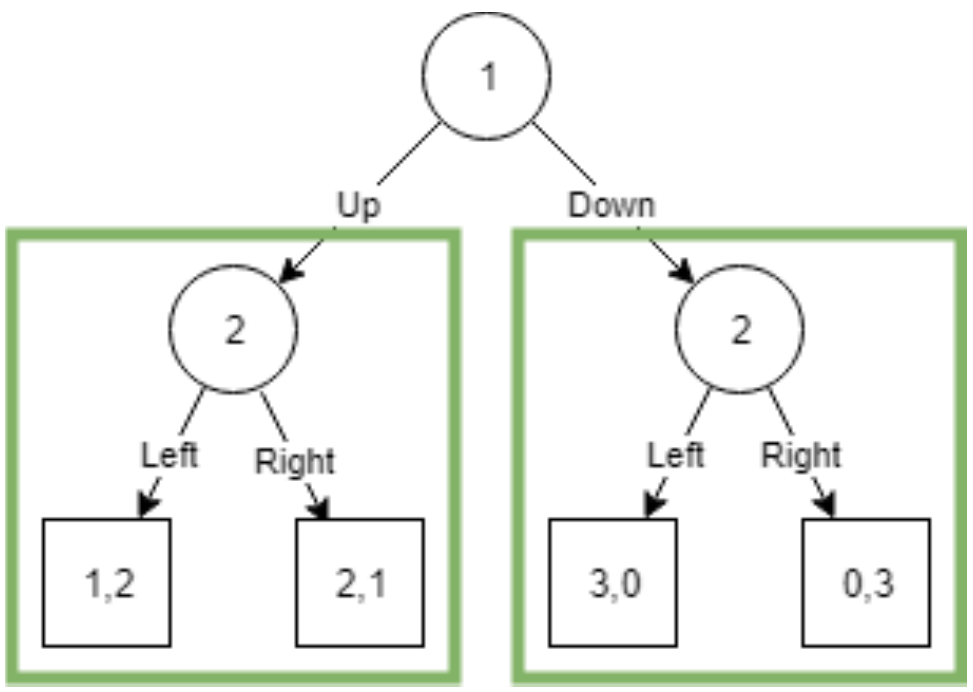
\includegraphics[width=0.75\textwidth]{figures/06SubgameExample01.png}
\end{figure}
\end{frame}

\begin{frame}
\frametitle{Examples of Subgames}
\begin{itemize}
\item Each of these green boxes contains a subgame.
\begin{itemize}
\item The smaller boxes are \alert{trivial subgames}, because they don't contain any meaningful choices.
\end{itemize}
\end{itemize}
\begin{figure}
\centering
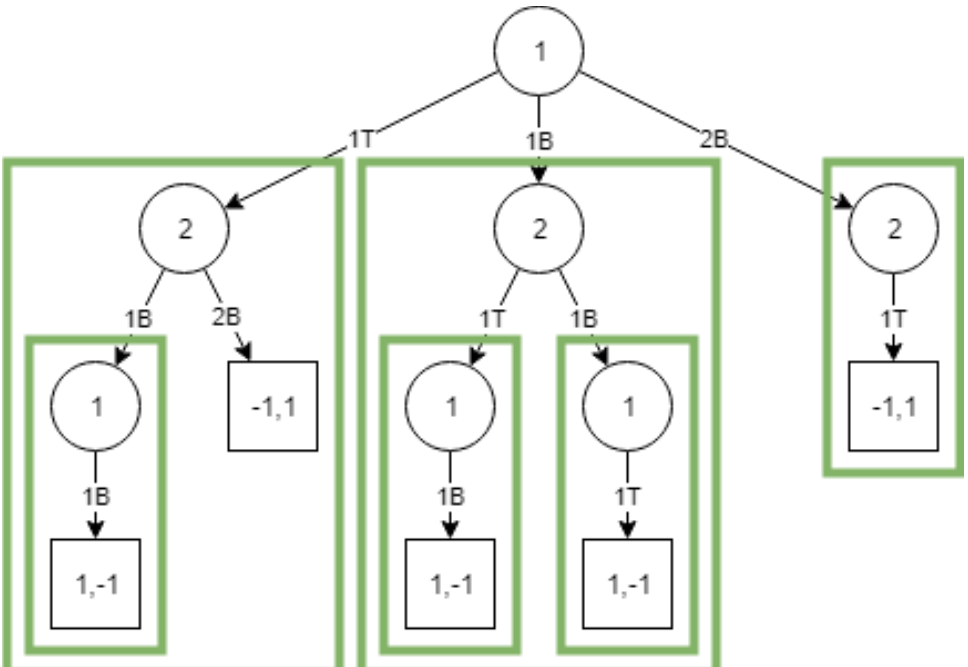
\includegraphics[width=0.75\textwidth]{figures/06SubgameExample02.png}
\end{figure}
\end{frame}

\begin{frame}
\frametitle{Examples of Subgames}
\begin{itemize}
\item A game is, technically, a subgame of itself, but it is an \alert{improper subgame}. (Any subgames other than the entire game are \alert{proper subgames}.)
\end{itemize}
\begin{figure}
\centering
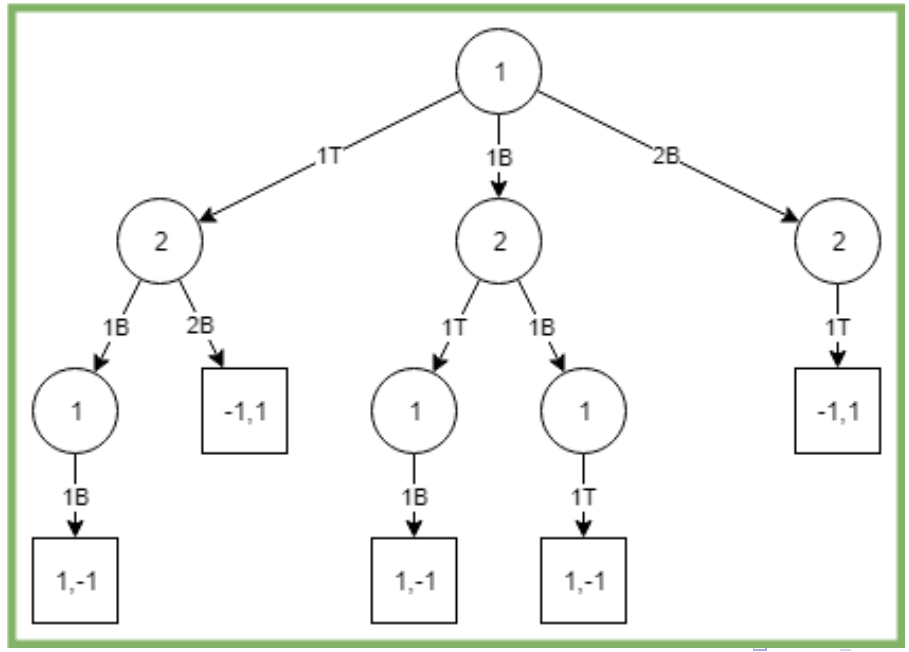
\includegraphics[width=0.7\textwidth]{figures/06SubgameExample03.png}
\end{figure}
\end{frame}

\begin{frame}
\frametitle{Subgame Perfection}
\begin{itemize}
\item So why do we care about subgames?
\item Because of a refinement of Nash equilibrium, called \alert{subgame-perfect Nash equilibrium}, that does not produce the questionable equilibria we saw earlier.
\item All subgame-perfect Nash equilibria are, obviously, regular Nash equilibria.
\item A subgame-perfect Nash equilibrium also has to produce a Nash equilibrium \textbf{in every subgame}.
\end{itemize}
\end{frame}

\begin{frame}
\frametitle{SPNE in the Entry Game}
\begin{itemize}
\item There is only a single proper subgame in the Entry Game.
\item A SPNE of this game must have a NE in that subgame.
\item The only NE of the subgame is for the Incumbent to Accommodate.
\end{itemize}
\begin{figure}
\centering
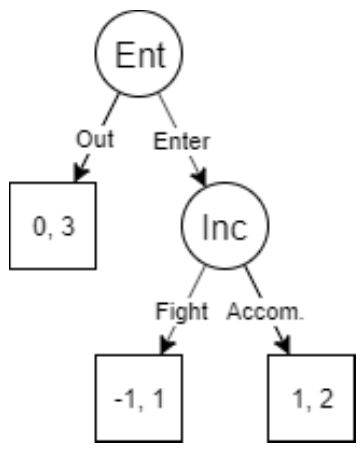
\includegraphics[width=.5\textwidth]{figures/08InferiorEntrant.png}
\end{figure}
\end{frame}

\begin{frame}
\frametitle{SPNE in the Entry Game}
\begin{itemize}
\item Given that the Incumbent Accommodates, the Entrant now faces a choice between staying Out, or Entering and being Accommodated.
\item The Entrant's best response is to Enter, and the SPNE is (Enter, Accommodate)
\end{itemize}
\begin{figure}
\centering
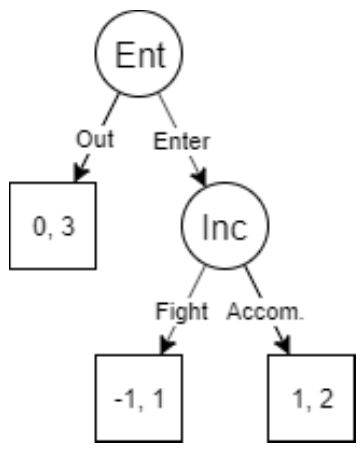
\includegraphics[width=.4\textwidth]{figures/08InferiorEntrant.png}
\end{figure}
\end{frame}

\begin{frame}
\frametitle{Rationality and Subgame Perfection}
\begin{itemize}
	\item To justify looking for SPNEs instead of NEs, we must make the assumption of \alert{commonly known sequential rationality}. There are two parts to this assumption:
	\begin{itemize}
		\item Players are aware that other players are sequentially rational.
		\item Knowing that other players are sequentially rational, each player can predict the others' rational behavior and will use this to choose an action which provides the largest possible payoff \textbf{at each node where they have a choice of actions}.
	\end{itemize}
	\item One way of thinking about this is that sequentially rational players choose their strategy ``on the fly," one move at a time, instead of all at once at the beginning of the game.
\end{itemize}
\end{frame}

\begin{frame}
\frametitle{Finding SPNEs: Backward Induction}
\begin{itemize}
\item The method for finding SPNEs is straightforward---we've already been using it without spelling it out formally.
	\begin{enumerate}
	\item Find all the decision nodes in the \textbf{lowest row} of decision nodes. (This assumes that the game tree is neat and orderly---which it will be if I'm giving you the game tree.)
	\item Find the optimal choice for players to make at each of these nodes, and mark the corresponding branch (or erase/cross out all the other branches).
	\item If you just solved the game's initial node, you're done! 
	\item Otherwise, identify all of the decision nodes in the \textbf{next row up} and return to step 2.
	\end{enumerate}
	\item At each step, remember to take into account the optimal moves that you've already found lower in the tree.
\end{itemize}
\end{frame}


\end{document}
